\section{Discussion}
\label{text:experiments/discussion}
The experiments above have shown the anticipative and safe-preserving capabilities of the proposed approach. In comparison to other state-of-the-art planning approaches it shows to better trade-off travel time with social compliance. Appropriate warm-starting of the optimization as well as attention filtering have shown to be key to make the approach runtime feasible, and find a locally optimal solution. Instead of failing to trade-off between the impacts on several pedestrians, which eventually leads to a poorer solution, only few (or one) pedestrians have to be considered. Consequently, the derived solution remains tractable with respect to the overall optimization. Next to tractability, generality over a wide range of prediction models is a key advantage of the proposed algorithm. While other state-of-the-art algorithms are limited to a simplifying set of assumptions about the pedestrian motion, or to self learned set of features such as \cite{Chen2017}\cite{vandenBerg2011}\cite{Ferrer2013}\cite{Kim2016}, the proposed algorithm is merely constrained by the availability of generative pedestrian prediction models. In particular, this gives raise to the opportunity to improve its performance with the availability of new prediction models. However, as shown in the following, being tightly-coupled to the performance of the prediction model also introduces adverse effects:
\newline
Although it enables the algorithm to find anticipative, safe-guarding while efficient robot trajectory, as shown, it poses high demands on the feasibility and accuracy of the underlying prediction model. Figure \ref{img:trajectron_misbehavior} illustrates a simple scenario, with only one pedestrian and the robot in the scene. It shows the predicted movement of the pedestrian, conditioned on four different planned trajectories of the robot. While the predictions 1-3 are very reasonable, the fourth prediction does not make sense intuitively. Here, the robot moves to the opposite direction of the pedestrian, i.e.\ , it increases the distance to the pedestrian as quick as possible. However, the pedestrian's movement is impact more than when the robot would just move in negative x-direction (third plot). This kind of unintentional and counterintuitive prediction becomes even more evident in the example displayed in Figure \ref{img:trajectron_misbehavior_2}. Here, the robot is planning a trajectory to pass behind the pedestrian, without affecting it much, since the pedestrian would already have passed when the robot would arrive there. As a reaction, intuitively, either an avoiding or an undisturbed movement would be expected. But instead, the prediction approaches the robot. 

\begin{figure}[!ht]
\begin{center}
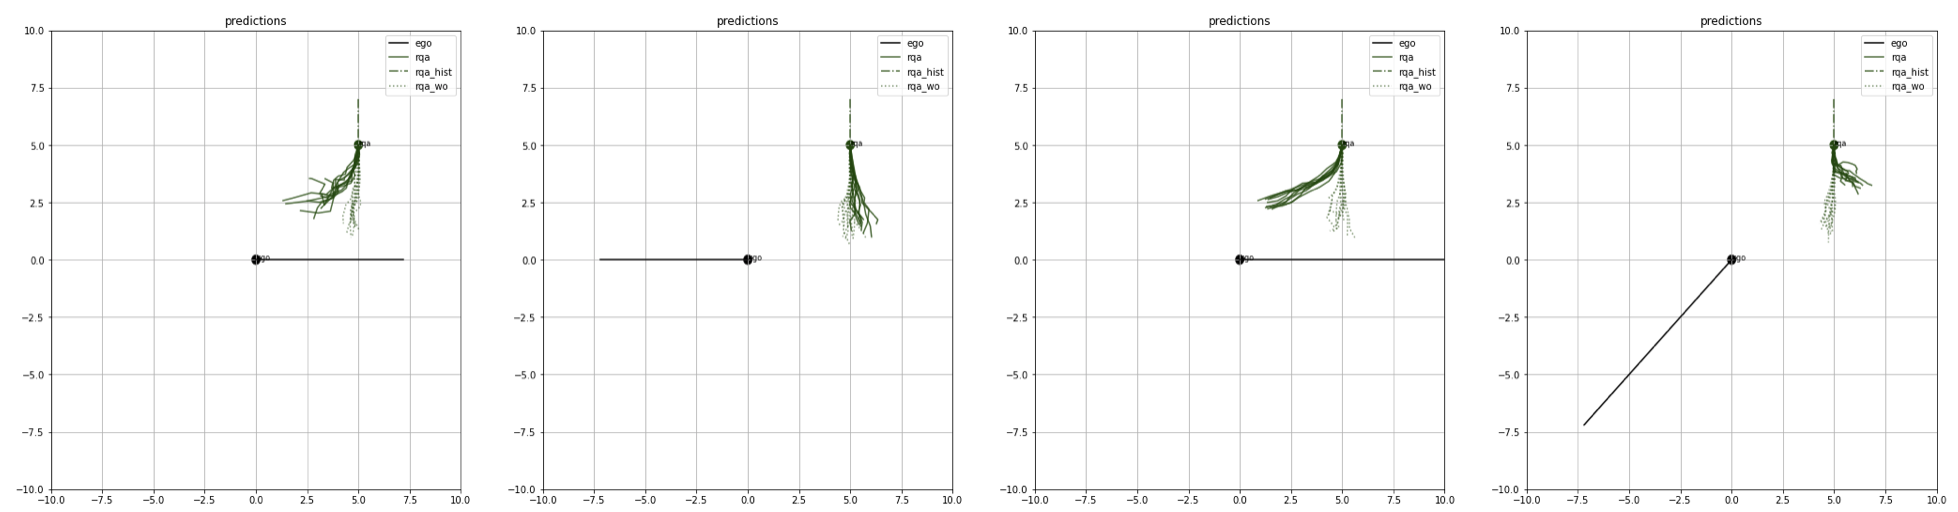
\includegraphics[width=\textwidth]{images/trajectron_misbehavior.png}
\captionof{figure}{Examples for unintentional predictions of Trajectron model \cite{Salzmann2020}. The dotted line ($rqa\_wo$) represents trajectory samples from the un-conditioned distribution, while the full line ($rqa$) displays trajectory samples which are conditioned on the respective robot movement.}
\label{img:trajectron_misbehavior}
\end{center}
\end{figure}

\begin{figure}[!ht]
\begin{center}
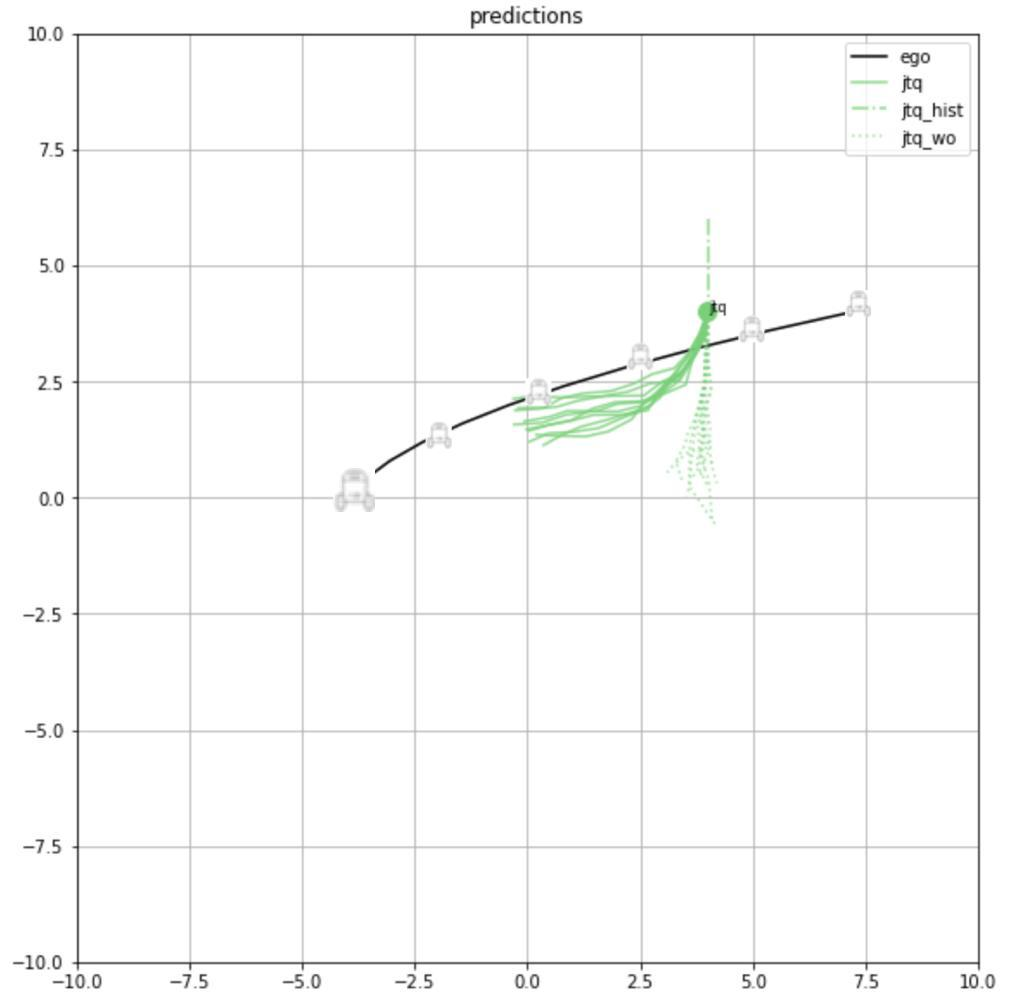
\includegraphics[width=0.5\textwidth]{images/trajectron_misbehavior_2.jpeg}
\captionof{figure}{Similarly to Figure \ref{img:trajectron_misbehavior}.}
\label{img:trajectron_misbehavior_2}
\end{center}
\end{figure}

According to one of the creators of the Trajectron model \cite{Salzmann2020}, this (counterintuitive) behavior could be reasoned in the type of data, the Trajectron model was trained on. Datasets as the ETH dataset \cite{Pellegrini2009} or the NuScenes dataset \cite{Caesar2020} are governed by largely structured environments, such as side- or crosswalks. In this context, counterintuitive predictions like in Figure \ref{img:trajectron_misbehavior_2} could originate from the limited amount of space the agents can move in. Then, the pedestrian is predicted to move in the direction of the robot, as the robot being there means that there is a walkable area. In this case, the problem could be fixed by introducing more structure in the environment, instead of assuming free-space. This was however out of the scope of the work, as it further complicates the trajectory optimization problem, and it thus left for future work. In any way, counterintuitive (or erroneous) pedestrian predictions are not only a problem for the algorithm, which was discussed in this work, but a core problem of all planning algorithms, which take into account predictions at all, such as the majority of model-based approaches presented in Chapter \ref{text:related}, such as \cite{Fox1997}\cite{Phillips2011}\cite{Knepper2012}\cite{Luo2018a}\cite{Nishimura2020a} and several more. Compared to these approaches however, the interactive formulation presented in this work is still an improvement, as it merely depends on the change of pedestrian behavior itself, instead of its explicit direction. Theoretically, the pedestrian going left or right in Figure \ref{img:trajectron_misbehavior_2} entails the same objective value, assuming that both behaviors imply a similar probability distribution for going straight. Consequently, the optimization may recover from these mis-predictions, by updating the robot trajectory to be more evasive.
\newline
Another drawback of the purposed approach is the (likely) non-convexity, non-linearity and partly intractability of the prediction model. The presented interactive-aware objective function generally might be hard to optimize, especially in case of phenomenological pedestrian prediction models. However, since the chosen objective formulation $J_{int}(\cdot)$ is a commonly used loss function for generative model, it has (at least empirically) shown great optimization performance, even for complex models. Comparable planning algorithm that are based on a prediction of a complex data-driven model, tend to be completely intractable, such as deep reinforcement learning-based approaches \cite{Knepper2012}\cite{Chen2017}\cite{Everett2018}. To determine the crucial elements and to define and trade-off core objectives of the optimization is here impossible. In contrary, by leveraging the prediction models internal structure within an optimization problem allows harnessing the full potential of data-driven models, while maintaining tractability at overall optimization-level.